\chapter{Marco Teórico}\label{marco-teorico}

\section{El Paradigma de Gestión de Producto y la Gestión de Proyecto}\label{el-paradigma-de-gestiuxf3n-de-producto-y-la-gestiuxf3n-de-proyecto}

Para llevar a cabo el diseño y la implementación del sistema de \eng{forecasting} para accidentes viales a nivel de producto mínimo viable (MVP) se debe comenzar observando el problema con una mirada amplia e integral, en el sentido de que este caso tiene una serie de particularidades las cuales restringen o condicionan el desarrollo respecto de un software tradicional. La gestión de un proyecto se mide o se juzga por el cumplimiento de las restricciones internas, es decir que si se termina a tiempo, respetando el alcance y dentro del presupuesto la gestión se considera exitosa o adecuada según el criterio de la triple restricción del PMI \autocite{pmi2021}. Ahora bien, este enfoque no resulta completamente representativo de los desafíos que implica implementar un sistema basado en inteligencia artificial que tiene como principal objetivo ser soporte para la toma de decisiones, esto es debido a que mientras un proyecto tiene un fin predeterminado un producto tecnológico posee un ciclo de vida dinámico que requiere iteración constante \autocite{cagan2018} e ir descubriendo y validando el producto a medida que se implementa en entornos reales.

Se tiene entonces un enfoque alternativo y de uso creciente en el mercado que es denominado Gestión de Producto (Product Management) que sugiere que el éxito de un proyecto depende de gestionar adecuadamente el impacto externo y el valor generado (\eng{outcomes}), es decir resolver un problema real del usuario u optimizar un proceso de la organización. Por otra parte se debe analizar la dimensión de la temporalidad, mientras que un proyecto tiene una naturaleza finita establecida por la fecha de inicio y la fecha de finalización, enfocarse en el producto implica asumir que el ciclo de vida es continuo y va evolucionando con las necesidades del usuario a través de mejoras y nuevas funcionalidades.

La siguiente característica notable que se debe tener en cuenta es el manejo de la incertidumbre y los requerimientos, en un proyecto generalmente se asume la predictibilidad en el sentido de que se intenta definir todo el alcance al principio del mismo, implementar un cambio implica un costo elevado e invertir tiempo en burocracia. Bajo el enfoque en el producto se asume la incertidumbre como constante, especialmente cuando se trabaja con software de inteligencia artificial. No se asume que se conoce lo que necesita o quiere el usuario sino que se lanzan prototipos y se mide la respuesta del usuario adaptando el rumbo con metodologías ágiles. Este último punto condiciona directamente la forma en la que se pueden constituir los equipos de trabajo, enfocarse en el proyecto requiere equipos temporales basados en la disponibilidad de recursos para esa tarea y enfocarse en el proceso permite equipos estables, multidisciplinarios capaces de desenvolverse con profundidad en el dominio del problema.

Este paradigma puede resumirse de la siguiente manera, un \eng{project manager} se enfoca en el cómo y cuándo coordinando recursos, mitigando riesgos de ejecución, eliminar bloqueos y asegurar el cronograma. Un \eng{product manager} en cambio se enfoca en el que y el por qué, entendiendo las necesidades del usuario, definiendo la visión a largo plazo, priorizando qué problemas resolver primero y alinear los objetivos del sistema con los del cliente.

El presente trabajo no adopta una postura excluyente entre ambos paradigmas ni los asume como los únicos existentes, sino que propone un enfoque híbrido que garantiza una efectiva adopción tecnológica por parte del usuario final al adaptar perfectamente el producto a sus necesidades y requerimientos al mismo tiempo que los conceptos y las herramientas de la gestión de proyectos permiten seleccionar la tecnología adecuada, identificar riesgos y restricciones, minimizar el uso de recursos y garantizar que no existan desviaciones significativas que condicionen la viabilidad del proyecto.

\section{Niveles de madurez tecnológica (ISO 16290:2013)}\label{niveles-de-madurez-tecnoluxf3gica-iso-162902013}

Originalmente, el concepto de TRL (technology readiness levels) o niveles de madurez tecnológica fue acuñado por la NASA en la década de los 70, sin embargo en 2013 la Organización Internacional de Estandarización formalizó este esquema publicando la norma internacional ISO 16290:2013, titulada \enquote{Sistemas espaciales --- Definición de los Niveles de Madurez Tecnológica (TRL) y sus criterios de evaluación}.

La finalidad de esta norma es proporcionar un lenguaje común y riguroso que permita a los investigadores, ingenieros y otras partes interesadas determinar correctamente el estado de desarrollo de una tecnología.

La estructura de la norma se divide en nueve niveles de madurez que inicia en el nivel 1 con la formulación de los principios básicos y culmina en el nivel 9 con un sistema probado y operando con éxito en un entorno real. Los primeros niveles abordan las etapas conceptuales iniciales de la investigación. En el nivel TRL 1 se identifican los principios científicos básicos que servirán como bases para el desarrollo posterior. En el nivel TRL 2, se formulan las aplicaciones prácticas de dichos principios y se definen los conceptos tecnológicos preliminares. Finalmente el nivel TRL 3 es el último de los niveles de la fase de investigación, donde se lleva a cabo la demostración analítica y experimental de las funciones del sistema mediante una prueba de concepto.

Los niveles desde TRL 4 hasta TRL 7 constituyen la etapa de desarrollo, donde en el TRL 4 se valida el funcionamiento de los componentes del sistema como un conjunto en un entorno de laboratorio para luego en TRL 5 incrementar la fidelidad de las pruebas, validando el funcionamiento en un entorno relevante y controlado. En TRL 6 se exige la demostración de funcionamiento del sistema en un entorno que simule la realidad donde el sistema debe evidenciar un funcionamiento predecible y documentado, para finalmente concluir con la etapa de desarrollo en el nivel TRL 7 donde un prototipo del sistema funcione en un entorno operativo real que garantice que el sistema es capaz de mitigar los riesgos asociados a la aplicación final antes de ser implementado definitivamente.

Finalmente, la escala de madurez de la norma culmina con los niveles orientados a la calificación formal y el uso continuado del sistema. En TRL 8 el sistema ha sido completamente finalizado y calificado para su uso mediante pruebas de aceptación que certifiquen el correcto funcionamiento. Por último, el nivel TRL 9 se alcanza únicamente cuando el sistema real ha sido probado con éxito y se encuentre disponible en el mercado listo para su uso generalizado.

La adopción de esta norma no solo justifica de manera estandarizada el estado actual del desarrollo alcanzado en el proyecto, sino que también traza una hoja de ruta para gestionar la incertidumbre técnica y asegurar la reproducibilidad del proceso de ingeniería implantado.

\section{Marco de referencia para el desarrollo de la IA (ISO 42001:2023)}\label{marco-de-referencia-para-el-desarrollo-de-la-ia-iso-420012023}

La norma internacional ISO 42001:2023, se titula \enquote{Tecnología de la información --- Inteligencia artificial --- Sistema de gestión} y se constituye como el primer estándar internacional dedicado a establecer los requisitos para la creación, implementación, mantenimiento y mejora continua de un sistema de gestión de inteligencia artificial. Su objetivo principal es estructurar un marco de trabajo que permita a las organizaciones desarrollar o utilizar sistemas de IA de forma ética, segura y transparente.

Para lograrlo, establece la obligatoriedad de realizar una evaluación de impacto del sistema para documentar y analizar las posibles consecuencias de implementar esta tecnología, así como también establece requisitos rigurosos para la gobernanza de datos, gestión del riesgo y la supervisión humana durante todo el ciclo de vida de la tecnología.

Otro aspecto importante de la norma es el énfasis en la calidad y procedencia de los datos, exigiendo procesos documentados para la preparación, selección y etiquetado de datos utilizados en el entrenamiento de modelos con la finalidad de evitar sesgos algorítmicos.

Además la norma también exige la identificación de las partes interesadas y la definición de políticas organizacionales que minimicen el impacto negativo de los sistemas de IA sobre los individuos y la sociedad.

Su estructura facilita la compatibilidad con otros marcos internacionales de gestión ya establecidos en las organizaciones, como la ISO 9001 para la calidad.

En el contexto de este proyecto, se buscará aplicarse la norma como una referencia a las buenas prácticas que facilite un enfoque ético y estructurado, por lo que su intención no es llegar al nivel requerido para una certificación.

Aunque el proyecto no busque una certificación técnica, se adoptarán los controles de la norma para gestionar la calidad y procedencia de los datos suministrados por el Ministerio Público Fiscal desde 2022, contribuyendo a que el entrenamiento de los modelos minimice errores que comprometan la toma de decisiones.

\section{Sistema de Alerta Temprana - SAT}\label{sistema-de-alerta-temprana---sat}

\subsection{Componentes del SAT}\label{componentes-del-sat}

Un sistema de alerta temprana se define como un conjunto de procesos estructurados e integrados que tiene por objetivo proveer al usuario, de manera anticipada la probabilidad de ocurrencia de un hecho o acontecimiento específico, ésta a veces puede ser una probabilidad pura y otras puede ser un indicador de probabilidad o riesgo relativo bajo diferentes tipos de formatos. En el contexto de este proyecto, el sistema de alerta temprana consiste en una arquitectura de \eng{forecasting} basada en varios modelos de inteligencia artificial que procesa datos históricos suministrados por el Ministerio Público Fiscal (MPF) para facilitar la toma de decisiones relacionadas con la asignación de recursos operativos.

Para diseñar un sistema de alerta temprana hay que tener en cuenta cuatro aspectos o componentes fundamentales que juntos explican cómo se relaciona con el problema para el cual fue concebido, estos son: Conocimiento del riesgo, seguimiento y pronóstico, comunicación y capacidad de respuesta.

En cuanto a el conocimiento del riesgo, esto está relacionado al contexto en el cual el sistema operará, es decir a la caracterización de la problemática y la comprensión de las variables que influyen en cómo se asignan recursos cuando suceden siniestros viales, que restricciones existen y qué mejoras podemos esperar luego de implementar el sistema.

Por otra parte tenemos que considerar el seguimiento y pronóstico, aquí se diseñará una arquitectura teniendo en cuenta todos los requisitos y las restricciones que contempla el producto. Se puede optar por modelos de línea de base puros como XGBoost, LightGBM o MLP configurados con hiperparámetros adaptados al procesamiento de series temporales para detección de anomalías y entrenados para hacer regresiones o clasificaciones. También se pueden incluir capas de decisión, que consisten en un post procesamiento determinista de la predicción (esto permite que el usuario ajuste la sensibilidad del SAT) para activar el sistema no solo en función de la salida del modelo sino que tenga en cuenta por ejemplo una capa estadística que usa una comparación Z-Score antes de dar el resultado. Otra alternativa que se contempló para hacer el \eng{forecasting} es el uso de múltiples modelos estructurados bajo una arquitectura de ensamblado ponderado (Weighted Ensemble), que le permitirá al SAT aprovechar las distintas ventajas de cada modelo para identificar patrones de distinta naturaleza y combinarlos en una única predicción. En este sentido es necesario comprender que para un mismo set de datos pueden existir modelos que capturen mejor dependencias de largo plazo, que capturen mejor la estacionalidad, que tengan funciones de probabilidad más suavizadas en la salida y otros que tengan gran explicabilidad como es el caso de los modelos basados en árboles de decisión.

Hasta el momento se tiene la capacidad de predecir el riesgo de ocurrencia de un hecho, en este caso un accidente, pero eso es solo una parte del sistema además hay que comunicar de alguna manera al tomador de decisiones. Este es un aspecto crítico de un sistema de alerta temprana porque hay que tener en cuenta en el diseño de experiencia de usuario que el mismo puede interpretar de distinta manera la predicción del modelo, generalmente se tiene la ventaja de que este será un experto en el dominio y tendrá una referencia basada en años de experiencia para comparar con la predicción, al mismo tiempo se tiene la desventaja de que es un usuario que no tiene conocimientos avanzados de estadística o de Machine Learning lo que hace casi obligatorio que el producto se implemente en un formato fácil de consumir como por ejemplo la codificación RAG (Red, Amber, Green).

El último componente que hay que tener en cuenta para diseñar un sistema de alerta temprana es la capacidad de respuesta, esto significa que cada tipo de alerta debe estar ligado a un plan de acción en concreto que debe llevar a cabo el personal del Ministerio Público Fiscal. Este punto excede el alcance de este trabajo en particular dada la complejidad y especificidad de los procesos que lleva a cabo tal institución. Queda pendiente para trabajos que pudieran realizarse en el futuro evaluar el impacto del sistema de \eng{forecasting} en el uso de recursos.

\subsection{Tipos de Alerta}\label{tipos-de-alerta}

Los tipos de alerta se pueden clasificar en dos grandes grupos, según su criticidad y según su horizonte temporal, a continuación se explicarán ambos tipos a fin de explicar cómo se deben tener en cuenta estos aspectos a la hora de diseñar un MVP.

La operativización de un SAT requiere la segmentación de las señales de riesgo mediante umbrales (\eng{thresholds}) basados en métricas estadísticas de control según el tipo de problema al que se está enfrentado y en ocasiones a las preferencias de los usuarios finales.

La metodología más validada tanto en el ámbito académico como en el mercado para escenarios similares consiste en segmentar según tres o cuatro niveles de riesgo con colores predefinidos como sigue:

\begin{description}
  \item[Nivel verde (línea de base).] Corresponde al estado estacionario del sistema. Los modelos predictivos proyectan que las variables se mantendrán dentro de los intervalos de confianza históricos y los límites de control aceptables.
  \item[Nivel amarillo (prevención).] Se activa ante la detección de desviaciones estadísticas sutiles o tendencias que indican una deriva del comportamiento normal. Este nivel no implica un riesgo inminente, sino la necesidad de que el tomador de decisiones se mantenga un poco más alerta.
  \item[Nivel naranja (alerta).] Se establece cuando los algoritmos determinan una alta probabilidad matemática de que las variables más significativas vulneren los umbrales de seguridad en un horizonte temporal cercano. Este nivel activa los procesos que el usuario haya predefinido o considere adecuados para esta alerta según su experiencia.
  \item[Nivel rojo (crítico).] Representa la inminencia o la ocurrencia efectiva del evento adverso. En este nivel, el sistema pone en conocimiento del usuario que está ante una anomalía significativa y que debe prepararse o tomar decisiones en proporción.
\end{description}

\subsection{Características de un SAT eficiente}\label{caracteruxedsticas-de-un-sat-eficiente}

La utilidad operativa de un SAT está condicionada por su horizonte de predicción. Los sistemas se dividen en dos categorías principales, las alertas inmediatas en tiempo real y las alertas predictivas por bloques o franjas de tiempo.

Las alertas inmediatas operan bajo un paradigma reactivo en tiempo real (\eng{near real-time}). Se configuran mediante algoritmos de detección de anomalías puntuales y se activan en el instante exacto en que un parámetro supera un límite preestablecido. Ofrecen una certidumbre matemática elevada respecto a la existencia del evento, pero reducen el margen de maniobra a cero dado que no le da tiempo suficiente al usuario para anticiparse y actuar.

Por otra parte, las alertas predictivas por bloques o franjas de tiempo discretas utilizan modelos supervisados o arquitecturas de aprendizaje profundo para proyectar la serie temporal hacia un horizonte futuro (próximos bloques de tiempo). Esta ventana temporal proporciona un diferencial de gran utilidad para la gestión de riesgos, permitiendo al usuario tomar decisiones anticipándose por medio de una estrategia de mitigación planificada.

El diseño a nivel algorítmico de un SAT basado en inteligencia artificial enfrenta una restricción metodológica conocida como el dilema entre la tasa de verdaderos positivos (\emph{recall}) y la tasa de valor predictivo positivo (precisión) \autocite{fawcett2006}.
% TODO(bib): en el original también se citaba "Saito y Rehmsmeier (2015)", que no figuraba en la lista de Bibliografía del documento original; agregarla a bibliografia.bib con sus datos completos.
Un sistema configurado y entrenado con una sensibilidad (\eng{recall}) extrema minimizará la ocurrencia de falsos negativos, asegurando la captura de cualquier anomalía, no obstante, incrementará exponencialmente los falsos positivos, induciendo el fenómeno operativo denominado fatiga de alertas, el cual degrada la confianza del usuario \autocite{ancker2017} dado que siempre está expuesto a una alerta. Por el contrario, la maximización de la precisión reduce las falsas alarmas, pero eleva el riesgo de perderse eventos críticos (falsos negativos) sin emitir alerta alguna. La calibración de los umbrales de decisión debe responder, por tanto, a una comprensión profunda de que implica alertar de cierta manera al tomador de decisiones, y cómo las mismas impactan en el servicio que estos prestan a los ciudadanos.

\section{Forecasting}\label{forecasting}

\subsection{Deep Learning y Machine Learning}\label{deep-learning-y-machine-learning}

En el campo del \eng{forecasting} para pronóstico basado en series temporales se pueden distinguir de manera predominante dos tecnologías para el tratamiento, procesamiento, y generación de modelos predictivos, por un lado tenemos al Aprendizaje Automático clásico o Machine Learning y por otro a Aprendizaje Profundo o Deep Learning. Además de la obvia distinción terminológica tenemos diferencias fundamentales en cómo estas técnicas procesan la información, usan diferentes arquitecturas a nivel algoritmos y tienen diferentes requisitos de infraestructura tecnológica que en ocasiones es determinante a la hora de elegir entre una o la otra.

El Machine Learning es una serie o conjunto de algoritmos y modelos que permiten a los sistemas identificar patrones como secuencias, anomalías, ciclos, grupos, tendencias y realizar inferencias a partir de datos sin que estos algoritmos sean programados explícitamente para cada tarea. En el contexto de este proyecto estas técnicas permiten implementar enfoques particularmente robustos dadas las características particulares que este dominio requiere y en especial puede aportar ventajas muy valoradas que se mencionan oportunamente.

Desde el punto de vista teórico, el Machine Learning se apalanca principalmente de la ingeniería de variables (\eng{feature engineering}), donde el conocimiento del dominio en este caso el referido a accidentología vial y su correspondiente proceso judicial permite extraer, construir y modelar características específicas para alimentar modelos como árboles de decisión, LightGBM o XGBoost. Este tipo de implementaciones tiene una ventaja muy relevante respecto de otras técnicas y tecnologías, y es que el Machine Learning tiene capacidad de Explicabilidad (XAI) al no operar como una caja negra absoluta, es decir que permitiría a los analistas judiciales, auditores, y usuarios en general comprender la lógica que subyace a una predicción, garantizando así que el producto esté alineado con los criterios de transparencia exigidos por la norma ISO/IEC 42001 (Cláusulas A.7.3 / A.7.4 / A.7.5).

El Deep Learning en cambio constituye una subdisciplina del Machine Learning inspirada en la estructura neurobiológica de una neurona del cerebro humano, utiliza redes neuronales artificiales constituidas por una capa de entrada, múltiples capas ocultas conectadas en simultáneo entre sí y estas últimas a una capa de salida que le permite aprender representaciones complejas de datos. A diferencia del Machine Learning clásico el Deep Learning tiene la capacidad intrínseca de realizar la extracción de características de forma automática, identificando relaciones no lineales y todo tipo de dependencias temporales profundas. Dentro del espectro del Deep Learning para series temporales se pueden destacar algunas arquitecturas como las redes de Perceptrón Multicapa (MLP) y las redes recurrentes LSTM (Long Short Term Memory) cada una de las cuales tiene requisitos y limitaciones específicas que se deben tener en cuenta antes de implementarlas.

\subsection{Árboles de decisión}\label{uxe1rboles-de-decisiuxf3n}

Un árbol de decisión es un modelo predictivo o una familia de modelos que segmenta el espacio de los datos de manera recursiva basándose en decisiones binarias, esto genera una estructura jerárquica de ramas y hojas que permite una representación intuitiva del proceso de decisión que favorece la explicabilidad del modelo. Estos árboles individuales suelen presentar limitaciones de varianza y riesgo de sobreajuste, estos inconvenientes pueden ser resueltos mediante el uso de diferentes técnicas como el ensamble mediante Boosting.

El método del Boosting consiste en plantear que un algoritmo de aprendizaje débil, es decir que puede predecir levemente mejor que realizar una predicción aleatoria, puede convertirse en un modelo con un gran rendimiento a través del uso de este método. Básicamente consiste en un método de aprendizaje por ensamble que combina una serie de aprendizajes poco asertivos para generar un modelo con una precisión elevada. Este entrenamiento es realizado de forma secuencial de manera que cada modelo corrige los errores cometidos por su predecesor, por ende la idea principal es combinar varios modelos individuales y unificarlos para mejorar la precisión general.

Existe una técnica de muy amplio uso en el campo del machine learning llamada Bagging que se explica a continuación. Tal metodología implica tomar los aprendizajes débiles para entrenar el modelo general en paralelo, de tal forma que se entrenan varios árboles de forma independiente y en simultáneo con distintos conjuntos de datos. El resultado final se obtiene mediante un promedio de las predicciones o una votación dependiendo de si el problema es de clasificación o regresión.

Si se quiere comparar estas dos metodologías se debe tener en cuenta que en el boosting el entrenamiento es secuencial y cada modelo trata de corregir los errores del modelo anterior, aumentando así la precisión global del estudio. Sin embargo, es más propenso al sobreajuste, por lo que es necesario tomar precauciones a la hora de incorporar nuevos árboles. Esta es una desventaja respecto al bagging y por eso, esta opción puede ser mejor para conjuntos de datos muy complejos con muchas observaciones atípicas.

\begin{figure}[htbp]
\centering
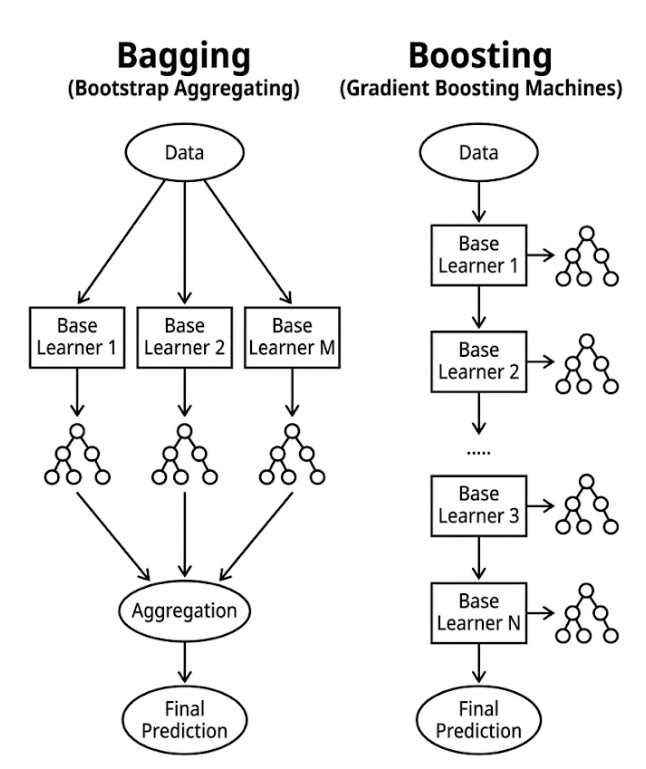
\includegraphics[width=0.59\linewidth]{imagenes/image10.png}
\caption{Arquitectura de bagging comparada con la de gradient boosting}
\label{fig:arquitectura-de-bootstrap-comparada-con-}
\notaflot{\fuentepropia{} en base a la arquitectura de Bagging y Boosting.}
\end{figure}

\subsection{LightGBM y XGBoost}\label{lightgbm-y-xgboost}

En el contexto de técnicas de aprendizaje supervisado las metodologías basadas en Gradient Boosting mencionadas anteriormente han ido evolucionando para optimizar su funcionamiento en lo referido a limitaciones computacionales en casos donde se necesita trabajar con volúmenes masivos de datos o problemas que tienen de base una alta dimensionalidad, por ejemplo proyectos en donde el modelo tienen que entrenar a partir de 65 características (columnas en el dataset) como lo es el caso de los datos originales de este proyecto de siniestros viales. Para resolver estas deficiencias surgieron arquitecturas optimizadas, las dos más notables son XGBoost (Extreme Gradient Boosting) y LightGBM (Light Gradient Boosted Machine) que destacan por incorporar innovaciones vitales en la función objetivo, la gestión del hardware y las estrategias de división de nodos.

Sobre XGBoost se menciona que fue desarrollado por Tianqi Chen y Carlos Guestrin en 2016, y es una implementación de alto desempeño de Gradient Boosting. Sus fortalezas se basan en dos pilares principales, la regularización matemática de la función objetivo y la optimización del sistema a nivel de hardware. A diferencia de otros modelos como GBM, XGBoost añade un término de regularización formal $\Omega$ a la función objetivo para controlar la complejidad y extensión de los árboles, esto evita el sobreajuste (\eng{overfitting}). La función objetivo se define según la \cref{eq:xgb-objetivo}:

\begin{equation}
\mathcal{L}^{(t)} = \sum_{i=1}^{n} l\left(y_i,\, \hat{y}_i^{(t-1)} + f_t(x_i)\right) + \Omega(f_t)
\label{eq:xgb-objetivo}
\end{equation}

Para optimizar esta función rápidamente con cualquier función de pérdida de segundo orden, XGBoost aplica una expansión en serie de Taylor de segundo grado. Esto permite que el algoritmo utilice tanto el gradiente de primer orden ($g_i$) como el gradiente de segundo orden (Hessiano, $h_i$), acelerando drásticamente la convergencia matemática.

\begin{equation}
\mathcal{L}^{(t)} \simeq \sum_{i=1}^{n} \left[ l\left(y_i,\, \hat{y}_i^{(t-1)}\right) + g_i f_t(x_i) + \tfrac{1}{2} h_i f_t^{2}(x_i) \right] + \Omega(f_t)
\label{eq:xgb-taylor}
\end{equation}

En cuanto a las características de este sistema hay algunos aspectos destacables a tener en cuenta, el primero de ellos es el soporte para valores faltantes (Sparsity-aware Split Finding) en el cual XGBoost asigna automáticamente una dirección por defecto en cada nodo para los datos ausentes basándose en cuál dirección minimiza la pérdida durante el entrenamiento. Otra es la estructura de bloques en paralelo, en esta los datos se almacenan en memoria en formato de bloques ordenados por columnas, esto permite calcular las divisiones de diferentes variables de forma paralela en la CPU. Por último se tiene acceso consciente en caché (Cache-aware Access) que le permite a XGBoost minimizar los fallos de caché asignando hilos de ejecución de manera que los gradientes se puedan leer en bloques continuos.

Por otra parte se tiene a LightGBM (Light Gradient Boosted Machine), el cual fue diseñado por Microsoft en 2017 y concebido específicamente para superar a XGBoost en velocidad de entrenamiento y consumo cuando se trabaja en proyectos de una gran dimensionalidad. De manera general se comenta que sus ventajas se basan en muestreo matemático y en una variante en la forma en la que crecen los árboles respecto del modelo antes mencionado.

Un aspecto fundamental que hay que distinguir cuando se implementan árboles en modelos predictivos es el referido al crecimiento por hojas (Leaf-wise) en contraposición al crecimiento por niveles (Level-wise). La mayoría de los algoritmos de boosting incluyendo las primeras versiones de XGBoost expanden los árboles a medida que van entrenando por el método de crecimiento por nivel, esto significa que todas las hojas de un nivel se generan simultáneamente manteniendo el árbol balanceado pero incurriendo en el riesgo de calcular divisiones ineficientes en ramas que tienen poco gradiente. LightGBM en cambio utiliza una estrategia distinta, el algoritmo busca y divide únicamente la hoja que genera mayor reducción de pérdida global, sin importar la profundidad. Este método genera árboles asimétricos y profundos que reducen rápidamente el error residual, siendo matemáticamente más eficientes a costa de tener una mayor tendencia a sobreajuste en muestras más chicas. LightGBM mitiga este efecto proporcionando un hiperparámetro que pone un límite estricto a la profundidad máxima del árbol.

\begin{table}[htbp]
\centering
\caption{Comparación entre XGBoost y LightGBM}
\label{tab:comparacion-xtreme-gradient-boosting-vs-}
\small
\begin{tabularx}{\textwidth}{@{}p{3.1cm}XX@{}}
\toprule
\textbf{Dimensión técnica} & \textbf{XGBoost} & \textbf{LightGBM} \\
\midrule
Estrategia de crecimiento & Normalmente \eng{level-wise} (por niveles) & \eng{Leaf-wise} (por hojas con mayor ganancia) \\
División de variables continuas & Percentiles ordenados (\eng{Weighted Quantile Sketch}) & Basado en histogramas optimizados (\eng{bins} fijos) \\
Manejo de \eng{sparse} & Algoritmo guiado por dispersión (\eng{sparsity-aware}) & Reducción por exclusión de características (EFB) \\
Técnica de muestreo & Muestreo aleatorio tradicional (\eng{subsampling}) & Muestreo unilateral por gradientes (GOSS) \\
Consumo de memoria RAM & Moderado-alto (guarda valores exactos o cuantiles complejos) & Extremadamente bajo (enteros de 8 bits para los \eng{bins}) \\
Velocidad de cómputo & Alta (optimización por bloques y caché) & Muy alta (GOSS, EFB e histogramas) \\
\bottomrule
\end{tabularx}
\notaflot{\fuentepropia{}, según comparación de XGBoost contra LightGBM.}
\end{table}

\subsection{Ventanas Deslizantes (Sliding Windows)}\label{ventanas-deslizantes-sliding-windows}

Comúnmente en los casos de aprendizaje automático que son más tradicionales los modelos asumen que en un determinado conjunto de datos tiene todos sus registros independientes y distribuidos uniformemente, esto significa por ejemplo que el orden en el cual se tienen los registros es irrelevante, que se tienen igual cantidad de etiquetas de cada clase cuando se quiere clasificar, entre otras implicaciones. Ahora bien, cuando se requiere hacer \eng{forecasting} o aplicar algún tipo de modelo predictivo para series temporales, los datos representan una dependencia cronológica que hace al fondo del problema, es decir, que de alguna manera el estado de una variable en el instante actual está condicionado o relacionado con sus estados cuantitativos en instantes previos. Para poder hacer uso de modelos como XGBoost, LightGBM o algún otro que se considere conveniente es obligatorio reestructurar el dataset de registros clásicos en formato tabla de hechos (Fact Table) a un formato matricial que capture esa estructura secuencial. El método que permite lograr este resultado es comúnmente conocido como enfoque de Ventanas Deslizantes, Sliding Windows, Lagging, o Ventanas de Retardo. Para el caso en específico de su uso en Machine Learning también se conoce como transformación de datos por formulación autorregresiva supervisada.

Dado que el tipo de problema que implica crear un sistema de \eng{forecasting} impulsado por inteligencia artificial para siniestros viales es de naturaleza multivariada se requerirá implementar el concepto de ventanas deslizantes para todas las características del dataset original. Específicamente se quiere decir que el número de víctimas o el riesgo de que existan accidentes en un tiempo determinado está relacionado con múltiples variables como lo pueden ser el clima, historial de siniestros previos, lugar, día y hora, festividades, etc, y que por lo tanto un registro deberá contener información tanto del presente como del pasado.

La aplicación del método de ventanas deslizantes en un entorno multivariado requiere una generalización geométrica y matemática del proceso de rezago (lagging), transformando tensores temporales en matrices tabulares aptas para algoritmos de aprendizaje automático. A continuación se formula el método mencionado ut supra.

Supóngase que se dispone de un sistema con $K$ variables distintas medidas simultáneamente a lo largo de $T$ instantes de tiempo. En cada paso de tiempo $t$ las observaciones no son un número escalar, sino un vector de observaciones $\mathbf{z}_t \in \mathbb{R}^{K}$:

\begin{equation}
\mathbf{z}_t = \left[ z_{t,1},\; z_{t,2},\; \dots,\; z_{t,K} \right]^{\top}
\label{eq:vector-observaciones}
\end{equation}

El conjunto de datos completo se representa como una secuencia cronológica de vectores o, equivalentemente, como una matriz de datos original $\mathbf{Z}$ de dimensiones $T \times K$:

\begin{equation}
\mathbf{Z} =
\begin{bmatrix}
\mathbf{z}_1^{\top} \\
\mathbf{z}_2^{\top} \\
\vdots \\
\mathbf{z}_T^{\top}
\end{bmatrix}
=
\begin{bmatrix}
z_{1,1} & z_{1,2} & \dots  & z_{1,K} \\
z_{2,1} & z_{2,2} & \dots  & z_{2,K} \\
\vdots  & \vdots  & \ddots & \vdots  \\
z_{T,1} & z_{T,2} & \dots  & z_{T,K}
\end{bmatrix}
\label{eq:matriz-datos}
\end{equation}

Este mecanismo convierte un flujo continuo multidimensional en una matriz plana estándar donde cada columna de la nueva matriz pasa a representar una entidad acoplada temporalmente. Puesto que esta transformación es de vital importancia para este proyecto se adjunta a continuación y a mera forma ilustrativa un cuadro que representa figurativamente el tratamiento que se le dio a los datos de accidentes viales.

\begin{longtable}[]{@{}lccccccc@{}}
\caption{Ilustración del método de retardos con ventana deslizante}
\label{tab:ilustracion-sobre-el-metodo-de-retardos-}\\
\toprule\noalign{}
\textbf{Fecha} & \textbf{Día} & \textbf{Temp} & \textbf{Lesiones} & \textbf{Inercia} & \textbf{Lagg\_1} & \textbf{Lagg\_3} & \textbf{Víctimas} \\
\midrule\noalign{}
\endfirsthead
\toprule\noalign{}
\textbf{Fecha} & \textbf{Día} & \textbf{Temp} & \textbf{Lesiones} & \textbf{Inercia} & \textbf{Lagg\_1} & \textbf{Lagg\_3} & \textbf{Víctimas} \\
\midrule\noalign{}
\endhead
\bottomrule\noalign{}
\endlastfoot
01/06 & L & 24 & 0 & 0 & 0 & 0 & 0 \\
02/06 & M & 24,5 & 0 & 0 & 0 & 0 & 0 \\
03/06 & X & 22 & 2 & 0 & 0 & 0 & 1 \\
04/06 & J & 23 & 0 & 1 & 1 & 1 & 0 \\
05/06 & V & 21,7 & 3 & 0 & 0 & 1 & 3 \\
06/06 & S & 20 & 2 & 2,2 & 3 & 4 & 1 \\
07/06 & D & 14,8 & 3 & 2,7 & 1 & 4 & 4 \\
08/06 & L & 12 & 0 & 3,1 & 4 & 8 & 0 \\
09/06 & M & 16,5 & 0 & 0 & 0 & 5 & 0 \\
10/06 & X & 22 & 0 & 0 & 0 & 4 & 0 \\
11/06 & J & 22,2 & 0 & 0 & 0 & 0 & 0 \\
12/06 & V & 21,9 & 3 & 0 & 0 & 0 & 1 \\
\end{longtable}

\notaflot{\fuentepropia{}.}

En la \cref{tab:ilustracion-sobre-el-metodo-de-retardos-} se puede observar cómo queda formateado un set de datos bajo la estructura de formulación autorregresiva supervisada, nótese que cada fila contiene información del presente como el día y la temperatura, e información del pasado como los retardos (laggs) y la inercia. Luego se registra la cantidad de víctimas bajo esas condiciones, el modelo que se use intentará predecir las víctimas conociendo el contexto disponible.

\subsection{AutoGluon y Transformers}\label{auto-gluon-y-transformers}

Existe un punto de tangencia entre la arquitectura Transformer (modelos con pesos pre entrenados a partir del cual se realiza un nuevo entrenamiento específico para el caso) y el ecosistema conocido como AutoGluon-TimeSeries (Auto Machine Learning) y es que la combinación de estas dos tecnologías genera un cambio de paradigma fundamental a la hora de realizar pronósticos de series temporales, superando la instancia de modelos estadísticos tradicionales y consolidando como estado del arte a modelos fundacionales de aprendizaje profundo global.

Los Transformers, son caracterizados por su mecanismo de auto atención escalada (scaled dot product attention) que les otorga una capacidad propia o intrínseca para capturar dependencias no lineales de largo plazo, y dinámicas cronológicas relativamente complejas sin verse comprometidos a nivel uso de memoria, o por el desvanecimiento del gradiente como es el caso de las primeras arquitecturas recurrentes.

Por otra parte AutoGluon para series temporales se beneficia de integrar de manera nativa arquitecturas basadas en atención, como la familia de modelos Chronos (Chronos 2, Chronos Bolt, etc) las cuales reestructuran el análisis numérico continuo propio de una serie temporal como una tarea de modelado de lenguaje autorregresivo, similar a los utilizados por los LLM (Large Language Model) actuales mediante procesos de escalamiento local y cuantización uniforme sobre un vocabulario de tokens.

La estrategia propuesta para el uso de AutoGluon no implica que un modelo único domine todos los escenarios reales posibles, es de suponer que según la naturaleza del problema que se enfrente, las limitaciones de información que se disponga, y el nivel de certidumbre requerida condicione la selección del modelo. Es por eso que el objetivo principal de esta tecnología es proveer al usuario una multiplicidad de modelos subdivididos en tres categorías estructurales que se definen a continuación.

Modelos Globales de Aprendizaje Profundo (Global Deep Learning): Modelos que comparten un único set de parámetros para todas las series temporales del dataset. Aquí se ubican los Transformers de secuencia como Chronos y PatchTST, y las redes neuronales recurrentes clásicas como DeepAR de GluonTS.

Modelos Locales Estadísticos (Local Statistical Models): Modelos univariados tradicionales que se ajustan de manera aislada e independiente para cada serie individual, como ARIMA, ETS y Theta de la librería Stats Forecast.

Modelos Tabulares Autoregresivos (Tree-Based Regressors): Mediante estrategias recursivas o por pasos, AutoGluon transforma las series a formato tabular mediante ventanas deslizantes según como se explicó en párrafos anteriores e inyecta estos datos en las arquitecturas optimizadas de LightGBM, XGBoost y CatBoost a través de AutoGluon-Tabular.

\subsection{Ensamble Ponderado (Weighted Ensemble)}\label{ensamble-ponderado-weighted-ensemble}

La fase final del algoritmo no consiste en seleccionar un único modelo individual con el mejor desempeño, sino en construir el denominado Ensamble Ponderado (Weighted Ensemble) que realiza la predicción final.

\begin{equation}
\hat{y}_{\text{ensemble}} = \sum_{m=1}^{M} w_m \cdot \hat{y}_m,
\qquad \text{sujeto a } \sum_{m=1}^{M} w_m = 1 \text{ y } w_m \geq 0
\label{eq:ensamble-ponderado}
\end{equation}

Esta última ecuación muestra que la predicción final es el resultado de agregar las predicciones de cada uno de los diferentes modelos según el peso ponderado que le asigna el método de AutoGluon.

De este modo el uso y la implementación de este modelo especializados para \eng{forecasting} en series temporales no solo es un software aislado sino que permite operativizar mediante un framework de trabajo la automatización del procesamiento de datos, la alineación temporal, el uso de transformers permitiendo el ajuste fino (modificaciones específicas al modelo original del transformer) y el ensamble ponderado final.

\begin{figure}[htbp]
\centering
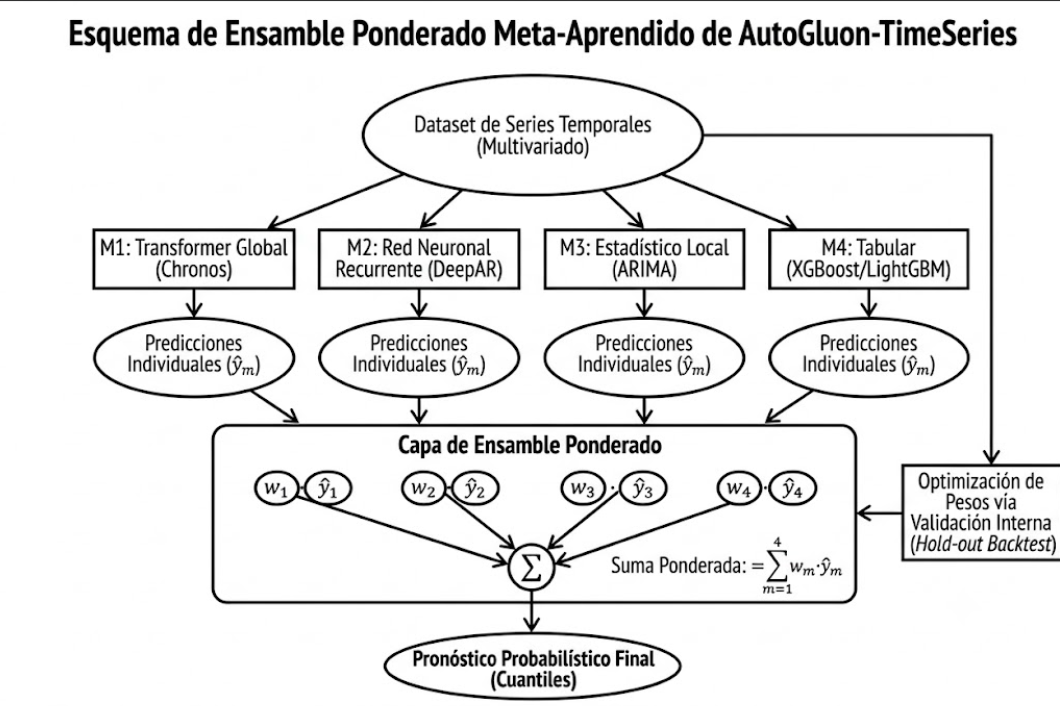
\includegraphics[width=\linewidth]{imagenes/image21.png}
\caption{Esquema del ensamble ponderado de AutoGluon}
\label{fig:esquema-de-ensamble-ponderado-de-autoglu}
\notaflot{\fuentepropia{} según la documentación del repositorio de AutoGluon-TimeSeries.}
\end{figure}
